%%%%%%%%%%%%%%%%%%%%%%%%%%%%%%%%
\clearpage
\section{Statistical framework}
\label{sec:statistics}
The observations in the hadronic and control regions described in 
chapter~\ref{sec:backgrounds} are interpreted through a likelihood model 
constructed in the following section. The method to set a limit on the 
cross-section of signal models is described in section~\ref{sec:cls}. 

%%%%%%%%%%%%%%%%%%%%%%%%%%%%%%%%
\subsection{Likelihood model\label{likelihood}}

\subsubsection{Hadronic sample}
\label{sec:hadronicLikelihood}

For a given \njet and \nb category, 
let $N$ be the number of bins of \HT. Let $n^i$ represent 
the number of events observed satisfying all selection requirements 
in each \HT bin $i$.  The likelihood of the observations can be written
as:
\begin{equation}
L_{hadronic}=\prod_i \mathrm{Pois}(n^i |\, b^i + s^i)
\label{eq:hadronicLikelihood}
\end{equation}

where $b^i$ represents the expected Standard Model background in bin
$i$, $s^i$ represents the expected number of signal events in bin $i$,
and $\mathrm{Pois}$ represents the Poisson distribution:

\begin{equation}
\mathrm{Pois}\left(k;\lambda\right)= \frac{\lambda^k \exp^{\left(-\lambda\right)}}{k!}
\label{eq:poisson}
\end{equation}

Due to the choice in \alphat and \scalht thresholds, the contribution 
from QCD events is expected to be negligible, Sec.~\ref{sec:alphat}. Therefore,
it is assumed that $b^i\equiv \ewk^i$ where $\ewk^i$ is the expected 
yield of electroweak events in bin $i$.


%%%%%%%%%%%%%%%%%%%%%%%%%%%%%%%%
%\subsection{\texorpdfstring{\HT}{HT} evolution models}
%\label{sec:htEvolutionModel}
%
%The hypothesis that for a process $p$ the $\alt$ ratio falls
%exponentially in \HT can be written this way:
%
%\begin{equation}
%R_{\alt}(\HT) = A e^{-k \HT}
%\end{equation}
%
%where $A$ and $k$ are parameters whose values will be determined.  Let
%$m_i$ represent the number of events observed with $\alt \le 0.55$ in
%each \HT bin $i$, and let \meanHt{i} represent the mean \HT of such
%events.  The expected background from the process is written thus:
%
%\begin{equation}
%b_{p}^{i} = \int_{x_i}^{x_{i+1}}\! \frac{\mathrm{d}N}{\mathrm{d}\HT}
%R_{\alt}\, \mathrm{d}\HT \quad , 
%\end{equation}
%
%where $\frac{\mathrm{d}N}{\mathrm{d}\HT}$ is the distribution of \HT
%for events with $\alt \le 0.55$, $x_i$ is the lower edge of the
%bin, and $x_{i+1}$ is the upper edge of the bin ($\infty$ for the
%final bin).  It is assumed that
%
%\begin{equation}
%\frac{\mathrm{d}N}{\mathrm{d}\HT}(x) = \sum_i
%m^{i}\delta(x-\meanHt{i}) \quad , 
%\end{equation}
%
%\ie within a bin the whole distribution occurs at the mean value of
%\HT in that bin. Then:
%
%\begin{equation}
%b_{p}^{i} = \int_{x_i}^{x_{i+1}}\! m^{i}\delta(x-\meanHt{i}) Ae^{-kx}\, \mathrm{d}x = m^{i} Ae^{-k \meanHt{i}} \quad .
%\label{eq:biDiracExp}
%\end{equation}
%

%%%%%%%%%%%%%%%%%%%%%%%%%%%%%%%%
\subsubsection{Electroweak control samples\label{sec:ewk}}

The electroweak background can be split into its reducible and 
irreducible backgrounds, i.e. $\ewk^i =  \zInv{i} + ttW^{i}$.
$\zInv{i}$ represents the contribution from \znunu + jets
events in \HT bin $i$ of the hadronically selected sample, 
and the variable $ttW^{i}$ represents the contribution from 
all other backgrounds in \HT bin $i$ of the hadronically 
selected sample.  
%Let \fZinv{i} represent the fraction of 
%\znunu + jets events in the total background $\ewk^{i}$. 
%It is a floating parameter limited between zero and one.
%Each contribution to the total electroweak re-written background can be 
%rewritten asLet:
%
%\begin{equation}
%  \zInv{i} \equiv \fZinv{i} \times \ewk^i 
%  \label{eq:ZinvEwk}
%\end{equation}
%
%\begin{equation}
%  ttW^{i} \equiv (1-\fZinv{i})\times \ewk^i
%  \label{eq:ttWEwk}
%\end{equation}
%
%The variable $\zInv{i}$ thus represents the expected number of \znunu
%events in \HT bin $i$ of the hadronically selected sample, and the
%variable $ttW^i$ represents the expected number of events from SM
%$W$-boson production (including top quark decays) ing \HT bin $i$ of
%the hadronically selected sample.

In each bin $i$ of \HT, there are two measurements: $n_{ph}^i$,
$n_{\mu}^i$, representing the event counts in the photon and single-muon.  
Each of these measurements has a corresponding yield in simulated 
data: $MC_{ph}^i$, $MC_{\mu}^i$.  The simulation also 
gives expected amounts of $\zInv{}$ and $t\bar{t}+W$ in 
the hadronically-selected sample: $MC_{\zInv{}}^i$ and 
$MC_{t\bar{t}+W}^i$.  After defining

\begin{equation}
r_{ph}^i = \frac{MC_{ph}^i}{MC_{\zInv{}}^i};\, r_{\mu}^i =
\frac{MC_{\mu}^i}{MC_{t\bar{t}+W}^i}\quad ,
\end{equation}

these likelihood functions are used:

\begin{equation}
\label{eq:photonLikelihood}
L_{ph}= \prod_i \mathrm{Pois}(n_{ph}^i |\, \rho_{phZ}^j \cdot
r_{ph}^{i} \cdot \zInv{i})
\end{equation}
%
%\begin{equation}
%\label{eq:mumuLikelihood}
%L_{\mu\mu}=\prod_i \mathrm{Pois}(n_{\mu\mu}^i |\, \rho_{\mu\mu Z}^j
%\cdot r_{\mu\mu}^{i} \cdot \zInv{i})
%\end{equation}
%
\begin{equation}
\label{eq:muonLikelihood}
L_{\mu}=\prod_i \mathrm{Pois}(n_{\mu}^i |\, \rho_{\mu W}^j \cdot
r_{\mu}^{i} \cdot ttW^{i} + s_{\mu}^i)\quad .
\end{equation}

Equation~\ref{eq:photonLikelihood} can be used to estimate the maximum
likelihood value for $\zInv{i}$ (the expectation for the \znunu\ +
jets background in the hadronic signal region) given the observations
$n_{ph}^i$ in the photon control sample and the ratios $r_{ph}^i$. A
similar construction is used when estimating $ttW^{i}$ from the single 
muon control sample (Equ.~\ref{eq:muonLikelihood}). The measurements in 
each of the control samples and the hadronic search region, along with 
the ratios $r_{ph}^{i}$ and $r_{\mu}^{i}$, are all considered
simultaneously through the relationship $\ewk^i =  \zInv{i} + ttW^{i}$.
The ratios $r_{ph}^{i}$ and $r_{\mu}^{i}$ are simply 
the inverse of the translation factor (1/TF) defined in 
Equ.~\ref{equ:pred-method} (Sec.~\ref{sec:background-method}). More 
specifically, $MC_{ph}^i$ and $MC_{\mu}^i$ are the yields obtained from MC
after applying the selection criteria for the photon and single muon samples, 
as defined by Equ.~\ref{equ:ratio-denom} (Sec.~\ref{sec:background-method}). 
The variables $MC_{t\bar{t}+W}^i$ and $MC_{\zInv{}}^i$ are defined by 
Equs.~\ref{equ:ratio-numer-gj} and~\ref{equ:ratio-numer-mj} 
(Sec.~\ref{sec:background-method}), respectively.

The parameters $\rho_{phZ}^j$ and $\rho_{\mu
  W}^j$ represent ``correction factors'' that accommodate the
systematic uncertainties associated with the control-sample-based
background constraints.  The quantities $\sigma_{phZ}^j$
and $\sigma_{\mu W}^j$ represent the relative
systematic uncertainties for the control sample constraints, taken
into account with the following terms:

\begin{equation}
\label{eq:ewkSyst}
L_{\rm EWK\, syst.}=\prod_j \mathrm{Logn}( 1.0 |\,\rho_{\mu W}^j,
\sigma_{\mu W}^j)\times \mathrm{Logn}( 1.0 |\,\rho_{ph Z}^j,
\sigma_{phZ}^j) \quad ,
\end{equation}

where Logn is the log-normal
distribution~\cite{cousins-log-normal}:

\begin{equation}
\label{eq:log-normal}
\mathrm{Logn}(x |\,\mu,\sigma_{\mathrm{rel.}}) =
\frac{1}{x\sqrt{2\pi}\ln{k}}\exp{\left(-\frac{\ln^2{\left(\frac{x}{\mu}\right)}}{2\ln^2{k}}\right)};\quad
k=1+\sigma_{\mathrm rel.}\quad. 
\end{equation}

One systematic parameter is assigned per \HT bin.

%\begin{table}\centering
%\caption{The systematic parameters used in \HT bins.  Left: categories
%  with up to eleven bins; right: category with four bins.}
%\label{tab:systMap}
%\footnotesize
%\begin{tabular}{lccccccccccc}
%\hline
%\hline
%\HT bin ($i$)         & 0 & 1 & 2 & 3 & 4 & 5 & 6 & 7 & 8 & 9 & 10 \\
%\hline
%syst. parameter ($j$) & 0 & 1 & 2 & 3 & 3 & 4 & 4 & 5 & 5 & 6 & 6 \\
%\hline
%\hline
%\end{tabular} \ \ 
%\begin{tabular}{lccccc}
%\hline
%\hline
%\HT bin ($i$)         & 0 & 1 & 2 & 3\\
%\hline
%syst. parameter ($j$) & 0 & 0 & 0 & 0\\
%\hline
%\hline
%\end{tabular}
%\end{table}
%
\newcommand{\rpi}{\ensuremath{r_{\mu}^{\prime\ i}}\xspace}

For the categories where $\nb=2$, the single muon sample is used to constrain the
total EWK background thus:

\begin{equation}
\rpi \equiv \frac{MC_{\mu}^i}{MC_{t\bar{t}+W+\zInv{}}^i}\quad ;
\end{equation}
\begin{equation}
\label{eq:muonLikelihoodTotalEwk}
L_{\mu}=\prod_i \mathrm{Pois}(n_{\mu}^i |\, \rho_{\mu W}^j \cdot
\rpi \cdot \ewk^{i} + s_{\mu}^i)\quad .
\end{equation}

The photon likelihood is dropped and splitting $\ewk^i$ is no longer
necessary thus $\zInv{i}$ and $ttW^{i}$ can be dropped. 

%%%%%%%%%%%%%%%%%%%%%%%%%%%%%%%%
\subsubsection{Contributions from signal}
\label{sec:signalContrib}

Let $x$ represent the cross section for a particular signal model, and
let $l$ represent the recorded luminosity.  Let $\epsilon^{i}_{had}$ 
be the analysis efficiency as simulated for the model in \HT bin $i$ 
of the hadronic sample.  Let $\delta$ represent the relative uncertainty on
the signal yield, assumed to be fully correlated among the bins, and
let $\rho_{sig}$ represent the ``correction factor'' to the signal
yield which accommodates this uncertainty.  Let $f$ represent an
unknown multiplicative factor on the signal cross section, for which
an allowed interval shall be determined.

Then the expected hadronic signal yield $s^i$ from
Equation~\ref{eq:hadronicLikelihood} is written as $s^i \equiv
f\rho_{sig} xl\epsilon_{had}^i$. The systematic uncertainty on
the signal efficiency is included via an additional term in the
likelihood:

\begin{equation}
L_{sig}=\mathrm{Logn}(1.0 |\,\rho_{sig}, \delta) \quad .
\end{equation}

%%%%%%%%%%%%%%%%%%%%%%%%%%%%%%%%
\subsubsection{Total likelihood}
\label{sec:totalLikelihood}

The likelihood function for a given selection $k$ is the product of
the terms described in the previous sections:

\begin{equation}
L^k = L_{hadronic}^k \times L_{\mu}^k \times L_{ph}^k \times
L_{\rm EWK\, syst.}^k \quad .
\end{equation}

A final reparametrization of the variables $\zInv{}$ and $ttW$ is made
by introducing, $f_{\rm Zinv}$, the fraction of \znunu + jets events in the total
electroweak background:

\begin{equation}
  \zInv{i} \equiv \fZinv{i} \times \ewk^i 
  \label{eq:ZinvEwk}
\end{equation}

\begin{equation}
  ttW^{i} \equiv (1-\fZinv{i})\times \ewk^i
  \label{eq:ttWEwk}
\end{equation}


This reparametrization allows representing the fit results with the floating
parameters $\ewk^{i}$ which is convenient for comparison to the observed data
in the hadronic region. 

In a category with 8 \HT bins and two control samples, there are 
32 nuisance parameters: $\{\ewk^{i}\}_{i=0}^{7}$, $\{\fZinv{i}\}_{i=0}^{7}$, $\{\rho_{phZ}\}_{i=0}^{7}$,
$\{\rho_{muZ}\}_{i=0}^{7}$. In the $\nb = 2$ categories there are 
18 nuisance parameters: $\{\ewk^{i}\}_{i=0}^{7}$, $\{\fZinv{i}\}_{i=0}^{7}$, 
$\{\rho_{muZ}\}_{i=0}^{7}$.  When considering signal, 
there is also the parameter $\rho_{sig}$; when multiple categories 
are fit simultaneously, the total likelihood is

\begin{equation}
L = L_{sig}\times \prod_k L_{hadronic}^k
\times L_{\mu}^k \times L_{ph}^k \times L_{\rm EWK\, syst.}^k \quad .
\end{equation}

\subsection{Limit setting\label{sec:cls}}

The following has been formulated in~\cite{LairdThesis} and is summarized 
here for completeness. 
Consider the likelihood ratio~\cite{Cowan:2010js}:

\begin{equation}
\label{eq:PLR}
\lambda(\mu) = \frac{ L(\mu,
\hat{\hat{\vec{\theta}}}) } {L(\hat{\mu}, \hat{\vec{\theta}}) } \;.
\end{equation}

Where $\hat{\hat{\vec{\theta}}}$ in the numerator denotes the
value of $\vec{\theta}$, the set of nuisance parameters in the likelihood,
that maximizes $L$ for the specified $\mu$.
The denominator is the maximized likelihood function, i.e., $\hat{\mu}$
and $\hat{\vec{\theta}}$ are their ML estimators. In the context of this
analysis $\mu \equiv f$ where $f$ is the signal strength as defined 
in section~\ref{sec:signalContrib}.  One can define the profile
likelihood ratio test statistic as~\cite{Cowan:2010js}:

\begin{equation}
\label{eq:qmu}
q_{\mu} =
\left\{ \! \! \begin{array}{ll}
               - 2 \ln \lambda(\mu)  & \hat{\mu} \le \mu  \;, \\*[0.2 cm]
               0 & \hat{\mu} > \mu \;,
              \end{array}
       \right.
\end{equation}

To test a specific signal model, one approach would be to perform many 
pseudo-experiments under the two separate hypotheses: background-only 
(i.e. $\mu=0$) and background with signal (i.e. $\mu=1$). $CL_{b}$ and 
$CL_{s+b}$~\cite{read,Junk} are defined as 1 - the quantile of $q_{\mu(obs)}$ in each of 
these distributions, where $q_{\mu(obs)}$ is the test statistic evaluated 
with the observed data. Figure~\ref{fig:hybrid_plot} illustrates two example distributions of
the test statistic under each hypothesis.  $CL_{s}$ is then defined as $CL_{s} \equiv CL_{s+b}/CL_{b}$, 
and a value $CL_{s} < 0.05$ excludes the signal hypothesis at 95\% confidence level. 

Another approach is to instead calculate the upper limit on the signal 
cross section by determining $f$ at $CL_{s} = 0.05$.  This approach samples 
CLs at varying signal strengths and the upper limit is 
determined through interpolation. If the upper limit on the cross section 
is lower than the nominal cross section, the signal model is excluded.

\begin{figure}[h!t]
  \begin{center}
      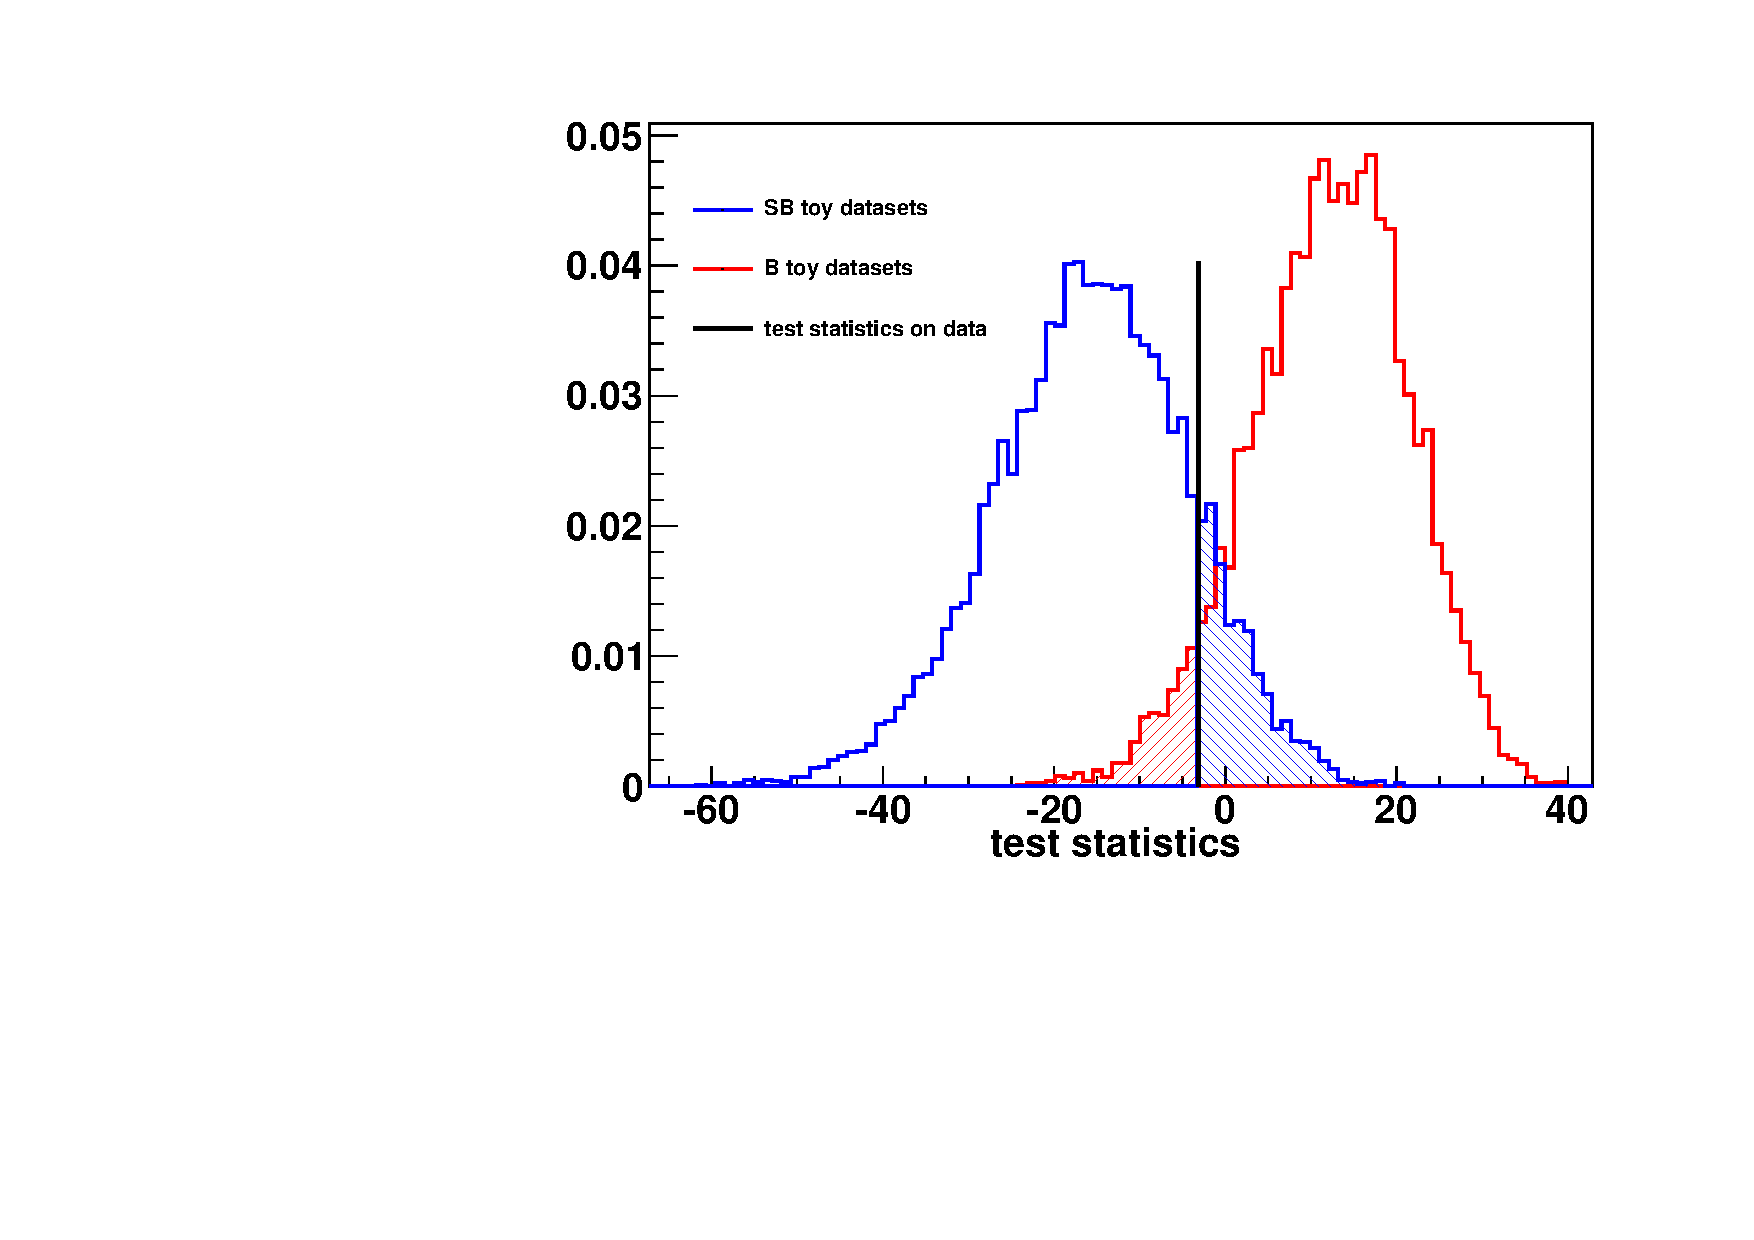
\includegraphics[width=0.45\textwidth,]{figures/hybrid_plot}
      \caption{\label{fig:hybrid_plot} The distributions of the test statistic $q_{\mu}$
        in the background-only (red, on the right) and signal+background (blue, on the left) hypotheses. 
        The black line represents the value of the $q_{\mu}$ on the tested data. The shaded areas represent 
        $1-CL_{b}$ (red) and $CL_{s+b}$ (blue).  From~\cite{Moneta:1289965}}.
    \label{fig:hybrid_plot}
  \end{center}
\end{figure}


